%%%%%%%%%%%%%%%%%%%%%%%%%%%%%%%%%%%%%%%%%%%%%%%%%%%%%%%%%%%%%%%
%
%     filename  = "Xuan_Dissertation.tex",
%     version   = "1.2.2",
%     date      = "2006/06/29",
%     authors   = "Gary L. Gray & Francesco Costanzo",
%     copyright = "Gary L. Gray & Francesco Costanzo",
%     address   = "Engineering Science and Mechanics,
%                  212 Earth & Engineering Sciences Bldg.,
%                  Penn State University,
%                  University Park, PA 16802,
%                  USA",
%     telephone = "814-863-1778 (GLG) or
%                  814-863-2030 (FC)",
%     email     = "gray@engr.psu.edu (GLG) or
%                  costanzo@engr.psu.edu (FC)",
%
%%%%%%%%%%%%%%%%%%%%%%%%%%%%%%%%%%%%%%%%%%%%%%%%%%%%%%%%%%%%%%%
%
% Change History:
%
% 1.2.2: * Added some information to the main driver file (this
%          file) regarding the use of hyperref with the
%          psuthesis class. Thanks to Nathan Urban for pointing
%          out the included workaround.
%
% 1.2.1: * Finally reproduced and fixed the problem where the
%          page number listed in the TOC for the Bibliography
%          was the last page number of the Bibliography.
%
%        * Added 10pt and 11pt options to the document class,
%          though we have no idea why anyone would want to use
%          such insanely small font sizes since it will lead to
%          line lengths that are much too long.
%
% 1.2.0: * Two additional class options have been added to
%          support honors theses submitted to the Schreyer
%          Honors College. These options are:
%             - honors
%             - honorsdepthead
%          See below for details.
%
%        * We have also added the commands:
%             - honorsdegreeinfo
%             - honorsadviser
%             - honorsdepthead
%          Again, see below for details.
%
% 1.1.2: * If you want to use the subfigure package with our
%          psuthesis class file, then you must must find the
%          following line in the psuthesis.cls file:
%
%          \RequirePackage{tocloft}
%
%          and add the subfigure option. We have already set
%          this up for you in the psuthesis.cls file to make
%          this easy to do.
%
% 1.1.1: * Added the fncychap package to the distribution.
%
% 1.1.0: * The way that the thesis frontmatter and backmatter
%          is generated has been completely re-done in order
%          to be more intuitive.
%        * We have added the ability to change the title of
%          the Dedication/Epigraph to anything you please.
%        * In the process of changing the format of the Table
%          of Contents to conform to the inflexible rules of
%          the Grad School (the word ``Chapter'' and
%          ``Appendix'' need to appear before the number and
%          letter, respectively), we have added an option to
%          the class called inlinechaptertoc that changes the
%          format of the Chapter/Appendix entries in the TOC.
%          Note that the tocloft package is now required.
%        * Appendices should now start with the
%          \Appendix command rather than \chapter. See the
%          accompanying files for examples.
%        * Added information regarding the Nontechnical
%          Abstract that is required of ESM students.
%        * Added the fncychap package for those of you who like
%          the nice Chapter headings it provides. We like
%          Lenny, but you don't have to use it if you don't
%          want to. In addition, the other options are: Sonny,
%          Glenn, Conny, Rejne, and Bjarne
%
% 1.0.4: * fixed the \addcontentsline entry for BibTeX within
%          the commented out text in the Bibliography section
%
% 1.0.3: * added a sigpage option to conform to new Grad School
%          requirements
%
% 1.0.2: * issued the \appendix command to start the appendices
%        * moved the \addcontentsline for the bibliography so
%          that the bibliography now shows up on the right page
%          in the TOC
%        * added some info if you use bibtex
%
% 1.0.1: * eqlist and eqparbox are now included in the archive
%
%%%%%%%%%%%%%%%%%%%%%%%%%%%%%%%%%%%%%%%%%%%%%%%%%%%%%%%%%%%%%%%
%
% This is a template file to help get you started using the
% psuthesis.cls for theses and dissertations at Penn State
% University. You will, of course, need to put the
% psuthesis.cls file someplace that LaTeX will find it.
%
% We have set up a directory structure that we find to be clean
% and convenient. You can readjust it to suit your tastes. In
% fact, the structure used by our students is even a little
% more involved and commands are defined to point to the
% various directories.
%
% This document has been set up to be typeset using pdflatex.
% About the only thing you will need to change if typesetting
% using latex is the \DeclareGraphicsExtensions command.
%
% The psuthesis document class uses the same options as the
% book class. In addition, it requires that you have the
% ifthen, calc, setspace, and tocloft packages.
%
% The first additional option specifies the degree type. You
% can choose from:
%     Ph.D. using class option <phd>
%     M.S. using class option <ms>
%     M.Eng. using class option <meng>
%     M.A. using class option <ma>
%     B.S. using class option <bs>
%     B.A. using class option <ba>
%     Honors Baccalaureate using the option <honors>
%
% If you specify either ba or bs in addition to honors, it will
% just use the honors option and ignore the ba or bs option.
%
% The second additional option <inlinechaptertoc> determines
% the formatting of the Chapter entries in the Table of
% Contents. The default sets them as two-line entries (try it).
% If you want them as one-line entries, issue the
% inlinechaptertoc option.
%
% The class option ``honors'' should be used for theses
% submitted to the Schreyer Honors College. This option
% changes the formatting on the Title page so that the
% signatures appear on the Title page. Be sure and comment
% out the command \psusigpage when using this option since it
% is not needed and it messes up the vertical spacing on the
% Title page.
%
% The class option ``honorsdepthead'' adds the signature of the
% department head on the Title page for those baccalaureate
% theses that require this.
%
% The class option ``secondthesissupervisor'' should be used
% for baccalaureate honors degrees if you have a second
% Thesis Supervisor.
%
% The vita is only included with the phd option and it is
% placed at the end of the thesis. The permissions page is only
% included with the ms, meng, and ma options.
%%%%%%%%%%%%%%%%%%%%%%%%%%%%%%%%%%%%%%%%%%%%%%%%%%%%%%%%%%%%%%%
% Only one of the following lines should be used at a time.
\documentclass[phd,11pt]{psuthesis}
\usepackage[T5]{fontenc}

\usepackage[utf8]{inputenc}

\usepackage[table, rgb]{xcolor}
\usepackage{caption}
\usepackage{subcaption}
\usepackage{tikz, pgfplots}

\usepackage{graphicx}
\usepackage{tikz}
\usetikzlibrary{arrows,decorations.pathmorphing,backgrounds,positioning,fit,petri}
\usepackage{tablefootnote, threeparttable, booktabs, multirow}
% \usepackage{algorithm, algorithmic}
\usepackage{algorithmicx}
\usepackage[ruled]{algorithm}
\usepackage{algpseudocode}

\usepackage{cite,url,bm,hyperref}
% \hypersetup{%
%     pdfborder = {0 0 0}
% }
%% ------------------end of block: tikz ----------------------------

\usetikzlibrary{shapes,arrows}

% \usepackage{subfig}
%%%%%%%%%%%%%%%%%%%%%%%%%%%%
% Packages we like to use. %
%%%%%%%%%%%%%%%%%%%%%%%%%%%%
\DeclareGraphicsExtensions{.pdf, .jpg}
\def\mb{\mathbf}
\def\xb{{\mathbf{x}}}
\def\yb{{\mathbf{y}}}

% \newcommand{\vect}[1]{\pmb{#1}}
% \newcommand{\mat}[1]{\pmb{#1}}
% \newcommand{\abs}[1]{\left|#1\right|}
% \newcommand{\norm}[1]{\left\|#1\right\|}
% \newcommand{\R}{\mathbb{R}}
% \newcommand{\Z}{\mathbb{Z}}

\definecolor{colorsrc}{rgb}{0.36, 0.54, 0.66}

% \definecolor{colornan}{rgb}{0.5, 0.5, 0.5}
% \definecolor{colornan}{rgb}{0.43, 0.21, 0.1}
% \definecolor{auburn}{rgb}{0.43, 0.21, 0.1}
% \definecolor{colorwnd2}{rgb}{1, .44, .37}
\definecolor{colorlcksvd}{rgb}{0.91, 0.84, 0.42}
\definecolor{colorlcksvdd}{rgb}{0.8, 0.0, 0.1}
\definecolor{colorlcksvd}{rgb}{1, 0.56, 0.0}
% \definecolor{colornan}{rgb}{0, 0.8, 0.0}
% \definecolor{colorsrc}{rgb}{0.5, 1, 0}
% \definecolor{colorfdd}{rgb}{0.6, 0.4, 0.8}
% \definecolor{colorfdd}{rgb}{0.93, 0.53, 0.18}
\definecolor{colorfddl}{rgb}{0.44, 0.16, 0.39}
\definecolor{colordlsi}{rgb}{0.55, 0.71, 0.0}
% \definecolor{colorlck}{rgb}{0.43, 0.21, 0.1}
% \definecolor{colorlck}{rgb}{0.89, 0.82, 0.04}
% \definecolor{colorlck}{rgb}{0.03, 0.27, 0.49}
\definecolor{colorcopar}{rgb}{0.9, .0, 0}
% \definecolor{colorlrsd}{rgb}{0.72, 0.53, 0.04}
\definecolor{colorjdl}{rgb}{0.0, 0.55, 0.55}
\definecolor{colordlr}{rgb}{0.0, 0.55, 0.55}
\definecolor{colorlrsdl}{rgb}{0.0, 0.2, 1.0} % blue
% \definecolor{colorlck}{rgb}{0.5, 0.5, 0.0}
% \definecolor{colorlck}{rgb}{0.0, 0.42, 0.24}
\definecolor{colorlck}{rgb}{0.0, 0.9, 0.9}
\definecolor{pinegreen}{rgb}{0.0, 0.47, 0.44}

\def\myaddplotlrsdl{\addplot+[thick, colorlrsdl, solid, mark = square*, mark size=1.4, mark options={colorlrsdl}]}
\def\myaddplotfddl{\addplot+[thick, colorfddl, mark = diamond*, mark size=1.4, mark options={colorfddl}]}
\def\myaddplotlcksvd{\addplot+[thick, colorlcksvd, mark = x, mark size=1.8, mark options={colorlcksvd}]}
\def\myaddplotlcksvdd{\addplot+[thick, green, mark = triangle, mark size=1.4, mark options={green}]}
\def\myaddplotdlsi{\addplot+[thick, colordlsi, mark = *, mark size=1.4, mark options={fill = white}]}
\def\myaddplotsrc{\addplot+[thick, colorsrc, mark = square, mark size=1.4, mark options={colorsrc}]}
\def\myaddplotcopar{\addplot+[thick, colorcopar, solid, mark = *, mark size=1.4, mark options={colorcopar}]}
\def\myaddplotjdl{\addplot+[thick, pinegreen, solid, mark = diamond*, mark size=1.4, mark options={pinegreen}]}
\def\myaddplotdlr{\addplot+[thick, cyan, solid, dashed, mark = triangle*, mark size=1.4, mark options={cyan}]}


% \def\myaddplotcopar{\addplot+[colorcopar, mark = square*, mark options={colorcopar}]}
% \def\myaddplotdfd{\addplot+[colordfd,  mark options={colordfd}]}
% \def\myaddplotfdd{\addplot+[colorfdd,  mark options={colorfdd}]}
% \def\myaddplotlck{\addplot+[colorlck,  mark options={colorlck}]}
% \def\myaddplotnan{\addplot+[colornan,  mark options={colornan}]}
% \def\myaddplotwnd{\addplot+[colorwnd,  mark options={colorwnd}]}
% \def\wnd{{black,fill=colorwnd}}

\def\x{{\mathbf x}}
\def\L{{\cal L}}

\newcommand{\vect}[1]{\mathbf{#1}}

\newcommand{\mat}[1]{\mathbf{#1}}
\newcommand{\abs}[1]{\left|#1\right|}
\newcommand{\norm}[1]{\left\|#1\right\|}
% \newcommand{\R}{\mathbb{R}}
\newcommand{\Z}{\mathbb{Z}}
\newcommand{\tb}{\textbf}


\def\bmt{\left[\begin{matrix}}
\def\dpcm{$\square$}
\def\emt{\end{matrix}\right]}
% \def\proof{\underline{Proof:}\\}
\def\dpcm{$\square$}
\def\half{\frac{1}{2}}
\def\imply{\Rightarrow}
\def\foralli{\forall i = 1, 2, \dots, n}
\def\im{\mathrm{im}}
\def\ker{\mathrm{ker}}
\def\eqv{\Leftrightarrow}
\def\tcg{\textcolor{newgreen}}
\def\mb{\mathbf}
\def\tb{\textbf}
\def\mb {\mathbf}
\def\mc {\mathcal}
\def\tcb{\textcolor{blue}}
\def\tcg{\textcolor{green}}
\def\tcr{\textcolor{red}}
\def\tcgr{\textcolor{gray}}
\def\bx{\mathbf{x}}
% \def\bW{\mathbf{W}}
\def\ba{\mathbf{a}}
\def\bb{\mathbf{b}}
\def\bc{\mathbf{c}}
\def\bd{\mathbf{d}}
\def\be{\mathbf{e}}
\def\fb{\mathbf{f}}
\def\bg{\mathbf{g}}
\def\bh{\mathbf{h}}
\def\bm{\mathbf{m}}
\def\M{\mathcal{M}}
\def\bp{\mathbf{p}}
\def\bq{\mathbf{q}}
\def\bs{\mathbf{x}}
\def\bu{\mathbf{u}}
\def\bv{\mathbf{v}}
\def\by{\mathbf{y}}
\def\bz{\mathbf{z}}
\def\and{\text{~and~}}
\def\barN{\bar{N}}
\def\barNi{\bar{N}_i}
\def\trace{\textrm{trace}}
\def\etal{\textit{et al.}}
\def\R{\mathbb{R}}

\def\bzeros{\mathbf{0}}

\def\bA{\mathbf{A}}
\def\bB{\mathbf{B}}
\def\bD{\mathbf{D}}
\def\bE{\mathbf{E}}
\def\Fb{\mathbf{F}}
\def\bG{\mathbf{G}}
\def\bL{\mathbf{L}}
\def\bH{\mathbf{H}}
\def\bI{\mathbf{I}}
\def\bJ{\mathbf{J}}
\def\bM{\mathbf{M}}
\def\bN{\mathbf{N}}
\def\bP{\mathbf{P}}
\def\bQ{\mathbf{Q}}
\def\bR{\mathbf{R}}
\def\bS{\mathbf{S}}
\def\bU{\mathbf{U}}
\def\bV{\mathbf{V}}
\def\bW{\mathbf{W}}
\def\bX{\mathbf{X}}

\def\bY{\mathbf{Y}}
\def\bZ{\mathbf{Z}}
\def\rank{\text{rank}}
\def\bDi{\mathbf{D}_i}
% \def\bSi{\mathbf{X}_i}
\def\bXi{\mathbf{X}_i}
% \def\bSi{\mathbf{X}_i}
\def\barX{\bar{\mathbf{X}}}
\def\barD{\bar{\mathbf{D}}}
\def\barX{\bar{\mathbf{X}}}
\def\barXi{\bar{\mathbf{X}}_i}
\def\barDi{\bar{\mathbf{D}}_i}
\def\barXi{\bar{\mathbf{X}}_i}
\def\bW{\mathbf{W}}
\def\bw{\mathbf{w}}

\def\la{\langle}
\def\ra{\rangle}

\def\bDc{\bD_{0}}
\def\bXc{\bX^{0}}
\def\mM{\mathcal{M}}
\def\wt{\widetilde}

\def\bbX{\lbar{\bX}}        
\def\bbx{\lbar{\bx}}        
\def\bbY{\lbar{\bY}}        
\def\bbD{\lbar{\bD}}  

%% ================== block: Slide footnotes ==========================
\def\footnoteSRC{\setcounter{footnote}{3}\footnote[frame]{\tiny J. Wright et al., Robust face recognition via sparse representation, IEEE TPAMI, 2009}}
\def\footnoteLLC{\setcounter{footnote}{4}\footnote[frame]{\tiny  H. Zhang et. al., Locality-constrained linear coding for image classification, CPVR 2010}}
\def\footnoteJSRC{\setcounter{footnote}{5}\footnote[frame]{\tiny  Yen, Multi-View Automatic Target Recognition using Joint Sparse Representation, Aerospace and Electronic Sys. 2012}}
\def\footnoteJDSRC{\setcounter{footnote}{6}\footnote[frame]{\tiny  J. Wang et. al., Joint dynamic sparse representation for multi-view face recognition,  PR 2012}}
\def\footnoteSHIRC{\setcounter{footnote}{7}\footnote[frame]{\tiny U. Srinivas et. al., Simultaneous sparsity model for histopathological image representation and classification, TMI 2014}}
\def\footnoteKSVD{\setcounter{footnote}{8}\footnote[frame]{\tiny  M. Elad et. al., K -SVD: An Algorithm for Designing Overcomplete Dictionaries for Sparse Representation, TSP 2006 }}
\def\footnoteODL{\setcounter{footnote}{9}\footnote[frame]{\tiny J. Mairal et. al., Online learning for matrix factorization and sparse coding, JMLR 2010}}
\def\footnoteDKSVD{\setcounter{footnote}{10}\footnote[frame]{\tiny  Q. Zhang, B. Li, Discriminative K-SVD for dictionary learning in face recognition, CVPR 2010 }}

\def\footnoteLCKSVD{\setcounter{footnote}{11}\footnote[frame]{\tiny  Z. Jiang et. al., Label consistent K-SVD: Learning a discriminative dictionary for recognition, TPAMI 2013}}
\def\footnoteFDDL{\setcounter{footnote}{12}\footnote[frame]{\tiny  M. Yang et. al., Fisher discrimination dictionary learning for sparse representation, ICCV 2011, IJCV 2014 }}
\def\footnoteDLR{\setcounter{footnote}{20}\footnote[frame]{\tiny  L. Li et. al., Learning low-rank and discriminative dictionary for image classification, Image and Vision Computing, 2014}}
\def\footnoteOMP{\setcounter{footnote}{13}\footnote[frame]{\tiny  Tropp et. al., Signal recovery from random measurements via orthogonal matching pursuit,  IEEE Transactions on Information Theory 2007}}
\def\footnoteNANDITA{\setcounter{footnote}{14}\footnote[frame]{\tiny N. Nayak et. al., Classification of tumor histopathology via sparse feature learning, ISBI 2013}}
\def\footnoteWNDCHARM{\setcounter{footnote}{15}\footnote[frame]{\tiny L. Shamir et. al., WNDCHARM--an open source utility for biological image analysis,  Source Code Biol. Med., 2008}}

\def\footnoteDFDLTMI{\setcounter{footnote}{16}\footnote[frame]{\tiny  \tcr{T. Vu} et. al., Histopathological Image Classification using Discriminative Feature-oriented Dictionary Learning, TMI 2015}}
\def\footnoteADMM{\setcounter{footnote}{17}\footnote[frame]{\tiny S. Boyd et. al., Distributed Optimization and Statistical Learning via the Alternating Direction Method of Multipliers, Foundations and Trends in Machine Learning, 2011}}
\def\footnoteFISTA{\setcounter{footnote}{18}\footnote[frame]{\tiny A. Beck et. al., A fast iterative shrinkage-thresholding algorithm for linear inverse problems, SIAM journal on Imaging sciences, 2009}}
\def\footnoteHojjatJPI{\setcounter{footnote}{19}\footnote[frame]{\tiny H. Mousavi \etal, Automated discrimination of lower and higher grade gliomas based on histopathological image analysis, JPI, 2015}}
% \def\footnote
% \def\footnoteDLSI{\setcounter{footnote}{3}\footnote[frame]{\tiny  I. Ramirez et. al., IEEE Computer Vision and Pattern Recognition (CVPR), 2010 }}






\def\footnotea{\setcounter{footnote}{3}\footnote[frame]{\tiny  H. Chang et. al., IEEE Transactions on Medical Imaging (TMI), 2013}}
\def\footnoteb{\setcounter{footnote}{4}\footnote[frame]{\tiny E. Ozdemir et. al., IEEE Transactions on Medical Imaging (TMI), 2013}}
\def\footnotec{\setcounter{footnote}{5}\footnote[frame]{\tiny M. Murat Dundar et. al., IEEE Transactions on Biomedical Engineering (TBME), 2011}}

\def\footnoteGDDL{\setcounter{footnote}{21}\footnote[frame]{\tiny  Suo et. al., Structured dictionary learning for classification, submitted to TSP 2014}}
\def\footnoteDLCORPA{\setcounter{footnote}{22}\footnote[frame]{\tiny S. Kong et. al., ECCV 2012}}
\def\footnoteDDLPC{\setcounter{footnote}{23}\footnote[frame]{\tiny  Guo et. al., ACCV 2012}}
\def\footnoteLPDDL{\setcounter{footnote}{24}\footnote[frame]{\tiny  Haghiri et. al., ICIP 2014}}
\def\footnoteDLSI{\setcounter{footnote}{25}\footnote[frame]{\tiny  Ramirez et. al., Classification and clustering via dictionary learning with structured incoherence and shared features, CVPR 2010}}
\def\footnoteDFDL{\setcounter{footnote}{26}\footnote[frame]{\tiny  T. Vu et. al., ISBI 2015}}
\def\footnoteDLRDSR{\setcounter{footnote}{27}\footnote[frame]{\tiny L. Ma et. al., CVPR 2012}}
\def\footnoteTDDL{\setcounter{footnote}{28}\footnote[frame]{\tiny J. Mairal et. al., ``Task-driven dictionary learning'', TPAMI, 2012}}
\def\footnoteTDDLLP{\setcounter{footnote}{29}\footnote[frame]{\tiny X. Sun, N. Nasrabadi, T. Tran, ``Task-driven dictionary learning for hyperspectral image classification with structured sparsity constraints'', TGRS, 2015}}
\def\footnoteJohn{\setcounter{footnote}{30}\footnote[frame]{\tiny J. Mckay, V. Monga \etal, Pose corrected sparsity for robust SONAR ATR, IGRSS, 2016}}



\def\diag{\text{diag}}


%% ------------------end of block: Slide footnotes ----------------------------



\newcommand{\myFormA}[1]{\bmt #1 & \bzeros & \dots & \bzeros \\ \bzeros & #1 & \dots & \bzeros \\ \dots & \dots & \dots & \dots \\ \bzeros & \bzeros & \dots & #1  \emt}
\newcommand{\myFormB}[1]{\bmt #1 & #1 & \dots & #1 \\ #1 & #1 & \dots & #1 \\ \dots & \dots & \dots & \dots \\ #1 & #1 & \dots & #1  \emt}

        
%% ========= long bar notation ==============================
\makeatletter
\newsavebox\myboxA
\newsavebox\myboxB
\newlength\mylenA
\newcommand*\lbar[2][.75]{%
    \sbox{\myboxA}{$\m@th#2$}%
    \setbox\myboxB\null% Phantom box
    \ht\myboxB=\ht\myboxA%
    \dp\myboxB=\dp\myboxA%
    \wd\myboxB=#1\wd\myboxA% Scale phantom
    \sbox\myboxB{$\m@th\overline{\copy\myboxB}$}%  Overlined phantom
    \setlength\mylenA{\the\wd\myboxA}%   calc width diff
    \addtolength\mylenA{-\the\wd\myboxB}%
    \ifdim\wd\myboxB<\wd\myboxA%
       \rlap{\hskip 0.5\mylenA\usebox\myboxB}{\usebox\myboxA}%
    \else
        \hskip -0.3\mylenA\rlap{\usebox\myboxA}{\hskip 0.3\mylenA\usebox\myboxB}%
    \fi}
\makeatother

\def\lbD{\lbar{\bD}}
\def\lbY{\lbar{\bY}}
\def\lbX{\lbar{\bX}}
% \def\lbX{\overline{\mathbf{X}}}
% \def\lbY{\overline{\mathbf{Y}}}

\usepackage[english]{babel}


%\documentclass[draft,phd,inlinechaptertoc]{psuthesis}
%\documentclass[draft,ms]{psuthesis}
%\documentclass[draft,honorsdepthead,honors]{psuthesis}
%\documentclass[draft,honors]{psuthesis}
%\documentclass[draft,secondthesissupervisor,honors]{psuthesis}
%\documentclass[draft,bs]{psuthesis}

%%%%%%%%%%%%%%%%%%%%%%%%%%%%
% Packages we like to use. %
%%%%%%%%%%%%%%%%%%%%%%%%%%%%
\usepackage{amsmath}
\usepackage{amssymb}
\usepackage{amsthm}
\usepackage{exscale}
\usepackage[mathscr]{eucal}
\usepackage{bm}
\usepackage{eqlist} % Makes for a nice list of symbols.
% \usepackage[final]{graphicx}
% \usepackage[dvipsnames]{color}
% \DeclareGraphicsExtensions{.pdf, .jpg,}
% \definecolor{colorsrc}{rgb}{0.36, 0.54, 0.66}

% \definecolor{colornan}{rgb}{0.5, 0.5, 0.5}
% \definecolor{colornan}{rgb}{0.43, 0.21, 0.1}
% \definecolor{auburn}{rgb}{0.43, 0.21, 0.1}
% \definecolor{colorwnd2}{rgb}{1, .44, .37}
\definecolor{colorlcksvd}{rgb}{0.91, 0.84, 0.42}
\definecolor{colorlcksvdd}{rgb}{0.8, 0.0, 0.1}
\definecolor{colorlcksvd}{rgb}{1, 0.56, 0.0}
% \definecolor{colornan}{rgb}{0, 0.8, 0.0}
% \definecolor{colorsrc}{rgb}{0.5, 1, 0}
% \definecolor{colorfdd}{rgb}{0.6, 0.4, 0.8}
% \definecolor{colorfdd}{rgb}{0.93, 0.53, 0.18}
\definecolor{colorfddl}{rgb}{0.44, 0.16, 0.39}
\definecolor{colordlsi}{rgb}{0.55, 0.71, 0.0}
% \definecolor{colorlck}{rgb}{0.43, 0.21, 0.1}
% \definecolor{colorlck}{rgb}{0.89, 0.82, 0.04}
% \definecolor{colorlck}{rgb}{0.03, 0.27, 0.49}
\definecolor{colorcopar}{rgb}{0.9, .0, 0}
% \definecolor{colorlrsd}{rgb}{0.72, 0.53, 0.04}
\definecolor{colorjdl}{rgb}{0.0, 0.55, 0.55}
\definecolor{colordlr}{rgb}{0.0, 0.55, 0.55}
\definecolor{colorlrsdl}{rgb}{0.0, 0.2, 1.0} % blue
% \definecolor{colorlck}{rgb}{0.5, 0.5, 0.0}
% \definecolor{colorlck}{rgb}{0.0, 0.42, 0.24}
\definecolor{colorlck}{rgb}{0.0, 0.9, 0.9}
\definecolor{pinegreen}{rgb}{0.0, 0.47, 0.44}

\def\myaddplotlrsdl{\addplot+[thick, colorlrsdl, solid, mark = square*, mark size=1.4, mark options={colorlrsdl}]}
\def\myaddplotfddl{\addplot+[thick, colorfddl, mark = diamond*, mark size=1.4, mark options={colorfddl}]}
\def\myaddplotlcksvd{\addplot+[thick, colorlcksvd, mark = x, mark size=1.8, mark options={colorlcksvd}]}
\def\myaddplotlcksvdd{\addplot+[thick, green, mark = triangle, mark size=1.4, mark options={green}]}
\def\myaddplotdlsi{\addplot+[thick, colordlsi, mark = *, mark size=1.4, mark options={fill = white}]}
\def\myaddplotsrc{\addplot+[thick, colorsrc, mark = square, mark size=1.4, mark options={colorsrc}]}
\def\myaddplotcopar{\addplot+[thick, colorcopar, solid, mark = *, mark size=1.4, mark options={colorcopar}]}
\def\myaddplotjdl{\addplot+[thick, pinegreen, solid, mark = diamond*, mark size=1.4, mark options={pinegreen}]}
\def\myaddplotdlr{\addplot+[thick, cyan, solid, dashed, mark = triangle*, mark size=1.4, mark options={cyan}]}


% \def\myaddplotcopar{\addplot+[colorcopar, mark = square*, mark options={colorcopar}]}
% \def\myaddplotdfd{\addplot+[colordfd,  mark options={colordfd}]}
% \def\myaddplotfdd{\addplot+[colorfdd,  mark options={colorfdd}]}
% \def\myaddplotlck{\addplot+[colorlck,  mark options={colorlck}]}
% \def\myaddplotnan{\addplot+[colornan,  mark options={colornan}]}
% \def\myaddplotwnd{\addplot+[colorwnd,  mark options={colorwnd}]}
% \def\wnd{{black,fill=colorwnd}}

\def\x{{\mathbf x}}
\def\L{{\cal L}}

\newcommand{\vect}[1]{\mathbf{#1}}

\newcommand{\mat}[1]{\mathbf{#1}}
\newcommand{\abs}[1]{\left|#1\right|}
\newcommand{\norm}[1]{\left\|#1\right\|}
% \newcommand{\R}{\mathbb{R}}
\newcommand{\Z}{\mathbb{Z}}
\newcommand{\tb}{\textbf}


\def\bmt{\left[\begin{matrix}}
\def\dpcm{$\square$}
\def\emt{\end{matrix}\right]}
% \def\proof{\underline{Proof:}\\}
\def\dpcm{$\square$}
\def\half{\frac{1}{2}}
\def\imply{\Rightarrow}
\def\foralli{\forall i = 1, 2, \dots, n}
\def\im{\mathrm{im}}
\def\ker{\mathrm{ker}}
\def\eqv{\Leftrightarrow}
\def\tcg{\textcolor{newgreen}}
\def\mb{\mathbf}
\def\tb{\textbf}
\def\mb {\mathbf}
\def\mc {\mathcal}
\def\tcb{\textcolor{blue}}
\def\tcg{\textcolor{green}}
\def\tcr{\textcolor{red}}
\def\tcgr{\textcolor{gray}}
\def\bx{\mathbf{x}}
% \def\bW{\mathbf{W}}
\def\ba{\mathbf{a}}
\def\bb{\mathbf{b}}
\def\bc{\mathbf{c}}
\def\bd{\mathbf{d}}
\def\be{\mathbf{e}}
\def\fb{\mathbf{f}}
\def\bg{\mathbf{g}}
\def\bh{\mathbf{h}}
\def\bm{\mathbf{m}}
\def\M{\mathcal{M}}
\def\bp{\mathbf{p}}
\def\bq{\mathbf{q}}
\def\bs{\mathbf{x}}
\def\bu{\mathbf{u}}
\def\bv{\mathbf{v}}
\def\by{\mathbf{y}}
\def\bz{\mathbf{z}}
\def\and{\text{~and~}}
\def\barN{\bar{N}}
\def\barNi{\bar{N}_i}
\def\trace{\textrm{trace}}
\def\etal{\textit{et al.}}
\def\R{\mathbb{R}}

\def\bzeros{\mathbf{0}}

\def\bA{\mathbf{A}}
\def\bB{\mathbf{B}}
\def\bD{\mathbf{D}}
\def\bE{\mathbf{E}}
\def\Fb{\mathbf{F}}
\def\bG{\mathbf{G}}
\def\bL{\mathbf{L}}
\def\bH{\mathbf{H}}
\def\bI{\mathbf{I}}
\def\bJ{\mathbf{J}}
\def\bM{\mathbf{M}}
\def\bN{\mathbf{N}}
\def\bP{\mathbf{P}}
\def\bQ{\mathbf{Q}}
\def\bR{\mathbf{R}}
\def\bS{\mathbf{S}}
\def\bU{\mathbf{U}}
\def\bV{\mathbf{V}}
\def\bW{\mathbf{W}}
\def\bX{\mathbf{X}}

\def\bY{\mathbf{Y}}
\def\bZ{\mathbf{Z}}
\def\rank{\text{rank}}
\def\bDi{\mathbf{D}_i}
% \def\bSi{\mathbf{X}_i}
\def\bXi{\mathbf{X}_i}
% \def\bSi{\mathbf{X}_i}
\def\barX{\bar{\mathbf{X}}}
\def\barD{\bar{\mathbf{D}}}
\def\barX{\bar{\mathbf{X}}}
\def\barXi{\bar{\mathbf{X}}_i}
\def\barDi{\bar{\mathbf{D}}_i}
\def\barXi{\bar{\mathbf{X}}_i}
\def\bW{\mathbf{W}}
\def\bw{\mathbf{w}}

\def\la{\langle}
\def\ra{\rangle}

\def\bDc{\bD_{0}}
\def\bXc{\bX^{0}}
\def\mM{\mathcal{M}}
\def\wt{\widetilde}

\def\bbX{\lbar{\bX}}        
\def\bbx{\lbar{\bx}}        
\def\bbY{\lbar{\bY}}        
\def\bbD{\lbar{\bD}}  

%% ================== block: Slide footnotes ==========================
\def\footnoteSRC{\setcounter{footnote}{3}\footnote[frame]{\tiny J. Wright et al., Robust face recognition via sparse representation, IEEE TPAMI, 2009}}
\def\footnoteLLC{\setcounter{footnote}{4}\footnote[frame]{\tiny  H. Zhang et. al., Locality-constrained linear coding for image classification, CPVR 2010}}
\def\footnoteJSRC{\setcounter{footnote}{5}\footnote[frame]{\tiny  Yen, Multi-View Automatic Target Recognition using Joint Sparse Representation, Aerospace and Electronic Sys. 2012}}
\def\footnoteJDSRC{\setcounter{footnote}{6}\footnote[frame]{\tiny  J. Wang et. al., Joint dynamic sparse representation for multi-view face recognition,  PR 2012}}
\def\footnoteSHIRC{\setcounter{footnote}{7}\footnote[frame]{\tiny U. Srinivas et. al., Simultaneous sparsity model for histopathological image representation and classification, TMI 2014}}
\def\footnoteKSVD{\setcounter{footnote}{8}\footnote[frame]{\tiny  M. Elad et. al., K -SVD: An Algorithm for Designing Overcomplete Dictionaries for Sparse Representation, TSP 2006 }}
\def\footnoteODL{\setcounter{footnote}{9}\footnote[frame]{\tiny J. Mairal et. al., Online learning for matrix factorization and sparse coding, JMLR 2010}}
\def\footnoteDKSVD{\setcounter{footnote}{10}\footnote[frame]{\tiny  Q. Zhang, B. Li, Discriminative K-SVD for dictionary learning in face recognition, CVPR 2010 }}

\def\footnoteLCKSVD{\setcounter{footnote}{11}\footnote[frame]{\tiny  Z. Jiang et. al., Label consistent K-SVD: Learning a discriminative dictionary for recognition, TPAMI 2013}}
\def\footnoteFDDL{\setcounter{footnote}{12}\footnote[frame]{\tiny  M. Yang et. al., Fisher discrimination dictionary learning for sparse representation, ICCV 2011, IJCV 2014 }}
\def\footnoteDLR{\setcounter{footnote}{20}\footnote[frame]{\tiny  L. Li et. al., Learning low-rank and discriminative dictionary for image classification, Image and Vision Computing, 2014}}
\def\footnoteOMP{\setcounter{footnote}{13}\footnote[frame]{\tiny  Tropp et. al., Signal recovery from random measurements via orthogonal matching pursuit,  IEEE Transactions on Information Theory 2007}}
\def\footnoteNANDITA{\setcounter{footnote}{14}\footnote[frame]{\tiny N. Nayak et. al., Classification of tumor histopathology via sparse feature learning, ISBI 2013}}
\def\footnoteWNDCHARM{\setcounter{footnote}{15}\footnote[frame]{\tiny L. Shamir et. al., WNDCHARM--an open source utility for biological image analysis,  Source Code Biol. Med., 2008}}

\def\footnoteDFDLTMI{\setcounter{footnote}{16}\footnote[frame]{\tiny  \tcr{T. Vu} et. al., Histopathological Image Classification using Discriminative Feature-oriented Dictionary Learning, TMI 2015}}
\def\footnoteADMM{\setcounter{footnote}{17}\footnote[frame]{\tiny S. Boyd et. al., Distributed Optimization and Statistical Learning via the Alternating Direction Method of Multipliers, Foundations and Trends in Machine Learning, 2011}}
\def\footnoteFISTA{\setcounter{footnote}{18}\footnote[frame]{\tiny A. Beck et. al., A fast iterative shrinkage-thresholding algorithm for linear inverse problems, SIAM journal on Imaging sciences, 2009}}
\def\footnoteHojjatJPI{\setcounter{footnote}{19}\footnote[frame]{\tiny H. Mousavi \etal, Automated discrimination of lower and higher grade gliomas based on histopathological image analysis, JPI, 2015}}
% \def\footnote
% \def\footnoteDLSI{\setcounter{footnote}{3}\footnote[frame]{\tiny  I. Ramirez et. al., IEEE Computer Vision and Pattern Recognition (CVPR), 2010 }}






\def\footnotea{\setcounter{footnote}{3}\footnote[frame]{\tiny  H. Chang et. al., IEEE Transactions on Medical Imaging (TMI), 2013}}
\def\footnoteb{\setcounter{footnote}{4}\footnote[frame]{\tiny E. Ozdemir et. al., IEEE Transactions on Medical Imaging (TMI), 2013}}
\def\footnotec{\setcounter{footnote}{5}\footnote[frame]{\tiny M. Murat Dundar et. al., IEEE Transactions on Biomedical Engineering (TBME), 2011}}

\def\footnoteGDDL{\setcounter{footnote}{21}\footnote[frame]{\tiny  Suo et. al., Structured dictionary learning for classification, submitted to TSP 2014}}
\def\footnoteDLCORPA{\setcounter{footnote}{22}\footnote[frame]{\tiny S. Kong et. al., ECCV 2012}}
\def\footnoteDDLPC{\setcounter{footnote}{23}\footnote[frame]{\tiny  Guo et. al., ACCV 2012}}
\def\footnoteLPDDL{\setcounter{footnote}{24}\footnote[frame]{\tiny  Haghiri et. al., ICIP 2014}}
\def\footnoteDLSI{\setcounter{footnote}{25}\footnote[frame]{\tiny  Ramirez et. al., Classification and clustering via dictionary learning with structured incoherence and shared features, CVPR 2010}}
\def\footnoteDFDL{\setcounter{footnote}{26}\footnote[frame]{\tiny  T. Vu et. al., ISBI 2015}}
\def\footnoteDLRDSR{\setcounter{footnote}{27}\footnote[frame]{\tiny L. Ma et. al., CVPR 2012}}
\def\footnoteTDDL{\setcounter{footnote}{28}\footnote[frame]{\tiny J. Mairal et. al., ``Task-driven dictionary learning'', TPAMI, 2012}}
\def\footnoteTDDLLP{\setcounter{footnote}{29}\footnote[frame]{\tiny X. Sun, N. Nasrabadi, T. Tran, ``Task-driven dictionary learning for hyperspectral image classification with structured sparsity constraints'', TGRS, 2015}}
\def\footnoteJohn{\setcounter{footnote}{30}\footnote[frame]{\tiny J. Mckay, V. Monga \etal, Pose corrected sparsity for robust SONAR ATR, IGRSS, 2016}}



\def\diag{\text{diag}}


%% ------------------end of block: Slide footnotes ----------------------------



\newcommand{\myFormA}[1]{\bmt #1 & \bzeros & \dots & \bzeros \\ \bzeros & #1 & \dots & \bzeros \\ \dots & \dots & \dots & \dots \\ \bzeros & \bzeros & \dots & #1  \emt}
\newcommand{\myFormB}[1]{\bmt #1 & #1 & \dots & #1 \\ #1 & #1 & \dots & #1 \\ \dots & \dots & \dots & \dots \\ #1 & #1 & \dots & #1  \emt}

        
%% ========= long bar notation ==============================
\makeatletter
\newsavebox\myboxA
\newsavebox\myboxB
\newlength\mylenA
\newcommand*\lbar[2][.75]{%
    \sbox{\myboxA}{$\m@th#2$}%
    \setbox\myboxB\null% Phantom box
    \ht\myboxB=\ht\myboxA%
    \dp\myboxB=\dp\myboxA%
    \wd\myboxB=#1\wd\myboxA% Scale phantom
    \sbox\myboxB{$\m@th\overline{\copy\myboxB}$}%  Overlined phantom
    \setlength\mylenA{\the\wd\myboxA}%   calc width diff
    \addtolength\mylenA{-\the\wd\myboxB}%
    \ifdim\wd\myboxB<\wd\myboxA%
       \rlap{\hskip 0.5\mylenA\usebox\myboxB}{\usebox\myboxA}%
    \else
        \hskip -0.3\mylenA\rlap{\usebox\myboxA}{\hskip 0.3\mylenA\usebox\myboxB}%
    \fi}
\makeatother

\def\lbD{\lbar{\bD}}
\def\lbY{\lbar{\bY}}
\def\lbX{\lbar{\bX}}
% \def\lbX{\overline{\mathbf{X}}}
% \def\lbY{\overline{\mathbf{Y}}}

\usepackage{caption}

\usepackage{epsf,psfig}
\usepackage{epsfig}
\usepackage{latexsym}
\usepackage{slashbox}

%%%%%%%%%%%%%%%%%%%%%%%%
% Setting for fncychap %
%%%%%%%%%%%%%%%%%%%%%%%%
% Comment out or remove the next two lines and you will get
% the standard LaTeX chapter titles. We like these A LOT
% better.
\usepackage[Lenny]{fncychap}
\ChTitleVar{\Huge\sffamily\bfseries}


%%%%%%%%%%%%%%%%%%%%%%%%%%%%%%%
% Use of the hyperref package %
%%%%%%%%%%%%%%%%%%%%%%%%%%%%%%%
%
% This is optional and is included only for those students
% who want to use it.
%
% To the hyperref package, uncomment the following line:
\usepackage{hyperref}
\hypersetup{%
    pdfborder = {0 0 0}
}
%
% Note that you should also uncomment the following line:
\renewcommand{\theHchapter}{\thepart.\thechapter}
%
% to work around some a problem hyperref has with the fact
% the psuthesis class has unnumbered pages after which page
% counters are reset.


%%%%%%%%%%%%%%%%%%%%%%%%%%%%%%%%%%%%
% SPECIAL SYMBOLS AND NEW COMMANDS %
%%%%%%%%%%%%%%%%%%%%%%%%%%%%%%%%%%%%
% \input{SupplementaryMaterial/UserDefinedCommands}


%%%%%%%%%%%%%%%%%%%%%%%%%%%%%%%%%%%%%%%%%
% Renewed Float Parameters              %
% (Makes floats fit better on the page) %
%%%%%%%%%%%%%%%%%%%%%%%%%%%%%%%%%%%%%%%%%
\renewcommand{\floatpagefraction}{0.85}
\renewcommand{\topfraction}      {0.85}
\renewcommand{\bottomfraction}   {0.85}
\renewcommand{\textfraction}     {0.15}
%\floatname{algorithm}{Procedure}
\renewcommand{\algorithmicrequire}{\textbf{Input:}}
\renewcommand{\algorithmicensure}{\textbf{Output:}}
% ----------------------------------------------------------- %

%%%%%%%%%%%%%%%%
% FRONT-MATTER %
%%%%%%%%%%%%%%%%
% Title
\title{Dictionary Learning for signal classification \\ under sparsity constraints}

% Author and Department
\author{Tiep Huu Vu}
\dept{Electrical Engineering}
% the degree will be conferred on this date
\degreedate{November 2015}
% year of your copyright
%\copyrightyear{2011}

% This command is used for students submitting a thesis to the
% Schreyer Honors College. The argument of this command should
% contain every after the word ``requirements'' that appears on
% the title page. This provides the needed flexibility for
% all the degree types.
\honorsdegreeinfo{for a baccalaureate degree \\ in Engineering Science \\ with honors in Engineering Science}

% This is the document type. For example, this could also be:
%     Comprehensive Document
%     Thesis Proposal
\documenttype{Ph.D. Dissertation Proposal}

% This will generally be The Graduate School, though you can
% put anything in here to suit your needs.
\submittedto{The Graduate School}


%%%%%%%%%%%%%%%%%%
% Signatory Page %
%%%%%%%%%%%%%%%%%%
% You can have up to 7 committee members, i.e., one advisor
% and up to 6 readers.
%
% Begin by specifying the number of readers.
\numberofreaders{3}

% For baccalaureate honors degrees, enter the name of your
% honors adviser below.
\honorsadviser{Honors P. Adviser}

% For baccalaureate honors degrees, if you have a second
% Thesis Supervisor, enter his or her name below.
\secondthesissupervisor{Second T. Supervisor}

% For baccalaureate honors degrees, certain departments
% (e.g., Engineering Science and Mechanics) require the
% signature of the department head. In that case, enter the
% name of your department head below.
\honorsdepthead{Department Q. Head}

% Input reader information below. The optional argument, which
% comes first, goes on the second line before the name.
\advisor[Thesis Advisor, Chair of Committee]
        {Vishal Monga}
        {Assistant Professor of Electrical Engineering}

\readerone[]
          {William E. Higgins}
          {Distinguished Professor of Electrical Engineering}

\readertwo[]
          {Kenneth Jenkins}
          {Professor of Electrical Engineering}

\readerthree[]
            {Robert T. Collins}
            {Associate Professor of Computer Science and Engineering}

%\readerfour[Optional Title Here]
%           {Reader Name}
%           {Professor of SomeThing}

%\readerfive[Optional Title Here]
%           {Reader Name}
%           {Professor of SomeThing}

% Makes use of LaTeX's include facility. Add as many chapters
% and appendices as you like.
% \includeonly{%
% Chapter-1/Chapter-1,%
% Chapter-2/Chapter-2,%
% Chapter-2/Chapter-2_2,%
% Chapter-3/Chapter-3,%
% Chapter-4/Chapter-4,%
% Chapter-5/Chapter-5,%
% Chapter-6/Chapter-6,%
% Appendix-A/Appendix-A%
% %Appendix-B/Appendix-B%
% }

%%%%%%%%%%%%%%%%%
% THE BEGINNING %
%%%%%%%%%%%%%%%%%
\begin{document}
%%%%%%%%%%%%%%%%%%%%%%%%
% Preliminary Material %
%%%%%%%%%%%%%%%%%%%%%%%%
% This command is needed to properly set up the frontmatter.
\frontmatter

%%%%%%%%%%%%%%%%%%%%%%%%%%%%%%%%%%%%%%%%%%%%%%%%%%%%%%%%%%%%%%
% IMPORTANT
%
% The following commands allow you to include all the
% frontmatter in your thesis. If you don't need one or more of
% these items, you can comment it out. Most of these items are
% actually required by the Grad School -- see the Thesis Guide
% for details regarding what is and what is not required for
% your particular degree.
%%%%%%%%%%%%%%%%%%%%%%%%%%%%%%%%%%%%%%%%%%%%%%%%%%%%%%%%%%%%%%
% !!! DO NOT CHANGE THE SEQUENCE OF THESE ITEMS !!!
%%%%%%%%%%%%%%%%%%%%%%%%%%%%%%%%%%%%%%%%%%%%%%%%%%%%%%%%%%%%%%

% Generates the signature page. This is not bound with your
% thesis.
%\psusigpage

% Generates the title page based on info you have provided
% above.
\psutitlepage

% Generates the committee page -- this is bound with your
% thesis. If this is an baccalaureate honors thesis, then
% comment out this line.
\psucommitteepage

% Generates the abstract. The argument should point to the
% file containing your abstract.
% \thesisabstract{SupplementaryMaterial/Abstract}

% Generates the Table of Contents
\thesistableofcontents

% Generates the List of Figures
% \thesislistoffigures

% Generates the List of Tables
% \thesislistoftables

% Generates the List of Symbols. The argument should point to
% the file containing your List of Symbols.
%\thesislistofsymbols{SupplementaryMaterial/ListOfSymbols}

% Generates the Acknowledgments. The argument should point to
% the file containing your Acknowledgments.
%\thesisacknowledgments{SupplementaryMaterial/Acknowledgments}

% Generates the Epigraph/Dedication. The first argument should
% point to the file containing your Epigraph/Dedication and
% the second argument should be the title of this page.
%\thesisdedication{SupplementaryMaterial/Dedication}{Dedication}



%%%%%%%%%%%%%%%%%%%%%%%%%%%%%%%%%%%%%%%%%%%%%%%%%%%%%%
% This command is needed to get the main part of the %
% document going.                                    %
%%%%%%%%%%%%%%%%%%%%%%%%%%%%%%%%%%%%%%%%%%%%%%%%%%%%%%
\thesismainmatter

%%%%%%%%%%%%%%%%%%%%%%%%%%%%%%%%%%%%%%%%%%%%%%%%%%
% This is an AMS-LaTeX command to allow breaking %
% of displayed equations across pages. Note the  %
% closing the "}" just before the bibliography.  %
%%%%%%%%%%%%%%%%%%%%%%%%%%%%%%%%%%%%%%%%%%%%%%%%%%
\allowdisplaybreaks{
%
%%%%%%%%%%%%%%%%%%%%%%
% THE ACTUAL CONTENT %
%%%%%%%%%%%%%%%%%%%%%%
% Chapters


% \include{Chapter-1/Chapter-1}
% %\include{Chapter-2/Chapter-2}
% \include{Chapter-3/Chapter-3}

%!TEX root = book.tex
\chapter{Linear Regression }

 
Trong bài này, tôi sẽ giới thiệu một trong những thuật toán cơ bản nhất (và đơn giản nhất) của Machine Learning. Đây là một thuật toán \textit{Supervised learning} có tên \textbf{Linear Regression} (Hồi Quy Tuyến Tính). Bài toán này đôi khi được gọi là \textit{Linear Fitting} (trong thống kê) hoặc \textit{Linear Least Square}. 

\section{Giới thiệu}
 
Quay lại \href{http://machinelearningcoban.com/2016/12/27/categories/#regression-hoi-quy}{ví dụ đơn giản được nêu trong bài trước}: một căn nhà rộng $x_1 ~ \text{m}^2$, có $x_2$ phòng ngủ và cách trung tâm thành phố $x_3~ \text{km}$ có giá là bao nhiêu. Giả sử chúng ta đã có số liệu thống kê từ 1000 căn nhà trong thành phố đó, liệu rằng khi có một căn nhà mới với các thông số về diện tích, số phòng ngủ và khoảng cách tới trung tâm, chúng ta có thể dự đoán được giá của căn nhà đó không? Nếu có thì hàm dự đoán $y = f(\mathbf{x}) $ sẽ có dạng như thế nào. Ở đây $\mathbf{x} = [x_1, x_2, x_3] $ là một vector hàng chứa thông tin \textit{input}, $y$ là một số vô hướng (scalar) biểu diễn \textit{output} (tức giá của căn nhà trong ví dụ này). 
 
\textbf{Lưu ý về ký hiệu toán học:} \textit{trong các bài viết của tôi, các số vô hướng được biểu diễn bởi các chữ cái viết ở dạng không in đậm, có thể viết hoa, ví dụ $x_1, N, y, k$. Các vector được biểu diễn bằng các chữ cái thường in đậm, ví dụ $\mathbf{y}, \mathbf{x}_1 $. Các ma trận được biểu diễn bởi các chữ viết hoa in đậm, ví dụ $\mathbf{X, Y, W} $.} 
 
Một cách đơn giản nhất, chúng ta có thể thấy rằng: i) diện tích nhà càng lớn thì giá nhà càng cao; ii) số lượng phòng ngủ càng lớn thì giá nhà càng cao; iii) càng xa trung tâm thì giá nhà càng giảm. Một hàm số đơn giản nhất có thể mô tả mối quan hệ giữa giá nhà và 3 đại lượng đầu vào là:  
 
 
$$y \approx  f(\mathbf{x}) = \hat{y}$$ 
$$f(\mathbf{x}) =w_1 x_1 + w_2 x_2 + w_3 x_3 + w_0 ~~~~ (1)$$ 
trong đó, $w_1, w_2, w_3, w_0$ là các hằng số,  $w_0$ còn được gọi là bias. Mối quan hệ $y \approx f(\mathbf{x})$ bên trên là một mối quan hệ tuyến tính (linear). Bài toán chúng ta đang làm là một bài toán thuộc loại regression. Bài toán đi tìm các hệ số tối ưu $ \\{w_1, w_2, w_3, w_0 \\}$ chính vì vậy được gọi là bài toán Linear Regression.  
 
\textbf{Chú ý 1:} $y$ là giá trị thực của \textit{outcome} (dựa trên số liệu thống kê chúng ta có trong tập \textit{training data}), trong khi $\hat{y}$ là giá trị mà mô hình Linear Regression dự đoán được. Nhìn chung, $y$ và $\hat{y}$ là hai giá trị khác nhau do có sai số mô hình, tuy nhiên, chúng ta mong muốn rằng sự khác nhau này rất nhỏ. 
 
\textbf{Chú ý 2:} \textit{Linear} hay \textit{tuyến tính} hiểu một cách đơn giản là \textit{thẳng, phẳng}. Trong không gian hai chiều, một hàm số được gọi là \textit{tuyến tính} nếu đồ thị của nó có dạng một \textit{đường thẳng}. Trong không gian ba chiều, một hàm số được goi là \textit{tuyến tính} nếu đồ thị của nó có dạng một \textit{mặt phẳng}. Trong không gian nhiều hơn 3 chiều, khái niệm \textit{mặt phẳng} không còn phù hợp nữa, thay vào đó, một khái niệm khác ra đời được gọi là \textit{siêu mặt phẳng} (\textit{hyperplane}). Các hàm số tuyến tính là các hàm đơn giản nhất, vì chúng thuận tiện trong việc hình dung và tính toán. Chúng ta sẽ được thấy trong các bài viết sau, \textit{tuyến tính} rất quan trọng và hữu ích trong các bài toán Machine Learning. Kinh nghiệm cá nhân tôi cho thấy, trước khi hiểu được các thuật toán \textit{phi tuyến} (non-linear, không phẳng), chúng ta cần nắm vững các kỹ thuật cho các mô hình \textit{tuyến tính}. 
 
 
 
 
 
\section{Phân tích toán học}
 
 
 
 
\subsection{Dạng của Linear Regression }
 
Trong phương trình $(1)$ phía trên, nếu chúng ta đặt $\mathbf{w} = [w_0, w_1, w_2, w_3]^T = $ là vector (cột) hệ số cần phải tối ưu và $\mathbf{\bar{x}} = [1, x_1, x_2, x_3]$ (đọc là \textit{x bar} trong tiếng Anh) là vector (hàng) dữ liệu đầu vào \textit{mở rộng}. Số $1$ ở đầu được thêm vào để phép tính đơn giản hơn và thuận tiện cho việc tính toán. Khi đó, phương trình (1) có thể được viết lại dưới dạng: 
 
$$y \approx \mathbf{\bar{x}}\mathbf{w} = \hat{y}$$ 
 
Chú ý rằng $\mathbf{\bar{x}}$ là một vector hàng. (\href{http://machinelearningcoban.com/math/#luu-y-ve-ky-hieu}{Xem thêm về ký hiệu vector hàng và cột tại đây}) 
 
 
 
\subsection{Sai số dự đoán }
 
Chúng ta mong muốn rằng sự sai khác $e$ giữa giá trị thực $y$ và giá trị dự đoán $\hat{y}$ (đọc là \textit{y hat} trong tiếng Anh) là nhỏ nhất. Nói cách khác, chúng ta muốn giá trị sau đây càng nhỏ càng tốt:  
 
$$ 
\frac{1}{2}e^2 = \frac{1}{2}(y - \hat{y})^2 = \frac{1}{2}(y - \mathbf{\bar{x}}\mathbf{w})^2 
$$ 
 
trong đó hệ số $\frac{1}{2} $ (\textit{lại}) là để thuận tiện cho việc tính toán (khi tính đạo hàm thì số $\frac{1}{2} $ sẽ bị triệt tiêu). Chúng ta cần $e^2$ vì $e = y - \hat{y} $ có thể là một số âm, việc nói $e$ nhỏ nhất sẽ không đúng vì khi $e = - \infty$ là rất nhỏ nhưng sự sai lệch là rất lớn. Bạn đọc có thể tự đặt câu hỏi: \textbf{tại sao không dùng trị tuyệt đối $ \|e\| $ mà lại dùng bình phương $e^2$ ở đây?} Câu trả lời sẽ có ở phần sau.  
 
 
 
 
 
 
\subsection{Hàm mất mát}
 
Điều tương tự xảy ra với tất cả các cặp \textit{(input, outcome)} $ (\mathbf{x}_i, y_i), i = 1, 2, \dots, N $, với $N$ là số lượng dữ liệu quan sát được. Điều chúng ta muốn, tổng sai số là nhỏ nhất, tương đương với việc tìm $ \mathbf{w} $ để hàm số sau đạt giá trị nhỏ nhất: 
 
$$ \mathcal{L}(\mathbf{w}) = \frac{1}{2}\sum_{i=1}^N (y_i - \mathbf{\bar{x}_i}\mathbf{w})^2 ~~~~~(2) $$  
 
Hàm số $\mathcal{L}(\mathbf{w}) $ được gọi là \textbf{hàm mất mát} (loss function) của bài toán Linear Regression. Chúng ta luôn mong muốn rằng sự mất mát (sai số) là nhỏ nhất, điều đó đồng nghĩa với việc  tìm vector hệ số $ \mathbf{w} $  sao cho  
giá trị của hàm mất mát này càng nhỏ càng tốt. Giá trị của $\mathbf{w}$ làm cho hàm mất mát đạt giá trị nhỏ nhất được gọi là \textit{điểm tối ưu} (optimal point), ký hiệu: 
 
$$ \mathbf{w}^* = \arg\min_{\mathbf{w}} \mathcal{L}(\mathbf{w})  $$  
 
Trước khi đi tìm lời giải, chúng ta đơn giản hóa phép toán trong phương trình hàm mất mát $(2)$. Đặt $\mathbf{y} = [y_1; y_2; \dots; y_N]$ là một vector cột chứa tất cả các \textit{output} của \textit{training data}; $ \mathbf{\bar{X}} = [\mathbf{\bar{x}}_1; \mathbf{\bar{x}}_2; \dots; \mathbf{\bar{x}}_N ] $ là ma trận dữ liệu đầu vào (mở rộng) mà mỗi hàng của nó là một điểm dữ liệu. Khi đó hàm số mất mát $\mathcal{L}(\mathbf{w})$ được viết dưới dạng ma trận đơn giản hơn: 
 
$$ 
\mathcal{L}(\mathbf{w})  
= \frac{1}{2}\sum_{i=1}^N (y_i - \mathbf{\bar{x}}_i\mathbf{w})^2 $$ 
$$ 
= \frac{1}{2} \|\mathbf{y} - \mathbf{\bar{X}}\mathbf{w} \|_2^2  
~~~(3) 
$$ 
 
với $ \| \mathbf{z} \|_2 $ là Euclidean norm (chuẩn Euclid, hay khoảng cách Euclid), nói cách khác $ \| \mathbf{z} \|_2^2 $ là tổng của bình phương mỗi phần tử của vector $\mathbf{z}$. Tới đây, ta đã có một dạng đơn giản của hàm mất mát được viết như phương trình $(3)$. 
 
 
 
 
 
\subsection{Nghiệm cho bài toán Linear Regression}
 
\textbf{Cách phổ biến nhất để tìm nghiệm cho một bài toán tối ưu (chúng ta đã biết từ khi học cấp 3) là giải phương trình đạo hàm (gradient) bằng 0!} Tất nhiên đó là khi việc tính đạo hàm và việc giải phương trình đạo hàm bằng 0 không quá phức tạp. Thật may mắn, với các mô hình tuyến tính, hai việc này là khả thi.  
 
Đạo hàm theo $\mathbf{w} $ của hàm mất mát là:  
$$ 
\frac{\partial{\mathcal{L}(\mathbf{w})}}{\partial{\mathbf{w}}}  
= \mathbf{\bar{X}}^T(\mathbf{\bar{X}}\mathbf{w} - \mathbf{y})  
$$ 
 
Các bạn có thể tham khảo bảng đạo hàm theo vector hoặc ma trận của một hàm số trong \href{https://ccrma.stanford.edu/~dattorro/matrixcalc.pdf}{mục D.2 của tài liệu này}. \textit{Đến đây tôi xin quay lại câu hỏi ở phần Sai số dự đoán phía trên về việc tại sao không dùng trị tuyệt đối mà lại dùng bình phương. Câu trả lời là hàm bình phương có đạo hàm tại mọi nơi, trong khi hàm trị tuyệt đối thì không (đạo hàm không xác định tại 0)}. 
 
Phương trình đạo hàm bằng 0 tương đương với:  
$$ 
\mathbf{\bar{X}}^T\mathbf{\bar{X}}\mathbf{w} = \mathbf{\bar{X}}^T\mathbf{y} \triangleq \mathbf{b}  
~~~ (4) 
$$ 
(ký hiệu $\mathbf{\bar{X}}^T\mathbf{y} \triangleq \mathbf{b} $ nghĩa là \textit{đặt} $\mathbf{\bar{X}}^T\mathbf{y}$ \textit{bằng} $\mathbf{b}$ ). 
 
Nếu ma trận vuông $ \mathbf{A} \triangleq \mathbf{\bar{X}}^T\mathbf{\bar{X}}$ khả nghịch (non-singular hay inversable) thì phương trình $(4)$ có nghiệm duy nhất: $ \mathbf{w} = \mathbf{A}^{-1}\mathbf{b}  $. 
 
Vậy nếu ma trận $\mathbf{A} $ không khả nghịch (có định thức bằng 0) thì sao? Nếu các bạn vẫn nhớ các kiến thức về hệ phương trình tuyến tính, trong trường hợp này thì hoặc phương trinh $ (4) $ vô nghiệm, hoặc làp  
nó 
có vô số nghiệm. Khi đó, chúng ta sử dụng khái niệm \href{https://vi.wikipedia.org/wiki/Giả_nghịch_đảo_Moore–Penrose}{\textit{giả nghịch đảo}} $ \mathbf{A}^{\dagger} $ (đọc là \textit{A dagger} trong tiếng Anh). (\textit{Giả nghịch đảo (pseudo inverse) là trường hợp tổng quát của nghịch đảo khi ma trận không khả nghịch hoặc thậm chí không vuông. Trong khuôn khổ bài viết này, tôi xin phép được lược bỏ phần này, nếu các bạn thực sự quan tâm, tôi sẽ viết một bài khác chỉ nói về giả nghịch đảo. Xem thêm: \href{http://www.sci.utah.edu/~gerig/CS6640-F2012/Materials/pseudoinverse-cis61009sl10.pdf}{Least Squares, Pseudo-Inverses, PCA \& SVD}.}) 
 
Với khái niệm giả nghịch đảo, điểm tối ưu của bài toán Linear Regression có dạng: 
 
 
$$ 
\mathbf{w} = \mathbf{A}^{\dagger}\mathbf{b} = (\mathbf{\bar{X}}^T\mathbf{\bar{X}})^{\dagger} \mathbf{\bar{X}}^T\mathbf{y} 
~~~ (5) 
$$ 
 
 
 
 
\section{Ví dụ trên Python}
 
 
\subsection{Bài toán}
 
Trong phần này, tôi sẽ chọn một ví dụ đơn giản về việc giải bài toán Linear Regression trong Python. Tôi cũng sẽ so sánh nghiệm của bài toán khi giải theo phương trình $(5) $ và nghiệm tìm được khi dùng thư viện \href{http://scikit-learn.org/stable/}{scikit-learn} của Python. (\textit{Đây là thư viện Machine Learning được sử dụng rộng rãi trong Python}). Trong ví dụ này, dữ liệu đầu vào chỉ có 1 giá trị (1 chiều) để thuận tiện cho việc minh hoạ trong mặt phẳng.  
 
Chúng ta có 1 bảng dữ liệu về chiều cao và cân nặng của 15 người như dưới đây: 
 
 
| Chiều cao (cm)     | Cân nặng (km)     | Chiều cao (cm)     | Cân nặng (kg)     | 
| :----------------: | :---------------: | :----------------: | :---------------: | 
| 147                | 49                | 168                | 60                | 
| 150                | 50                | 170                | 72                | 
| 153                | 51                | 173                | 63                | 
| 155                | 52                | 175                | 64                | 
| 158                | 54                | 178                | 66                | 
| 160                | 56                | 180                | 67                | 
| 163                | 58                | 183                | 68                | 
| 165                | 59                |                    |                   | 
 
 
Bài toán đặt ra là: liệu có thể dự đoán cân nặng của một người dựa vào chiều cao của họ không? (\textit{Trên thực tế, tất nhiên là không, vì cân nặng còn phụ thuộc vào nhiều yếu tố khác nữa, thể tích chẳng hạn}). Vì blog này nói về các thuật toán Machine Learning đơn giản nên tôi sẽ giả sử rằng chúng ta có thể dự đoán được. 
 
Chúng ta có thể thấy là cân nặng sẽ tỉ lệ thuận với chiều cao (càng cao càng nặng), nên có thể sử dụng Linear Regression model cho việc dự đoán này. Để kiểm tra độ chính xác của model tìm được, chúng ta sẽ giữ lại cột 155 và 160 cm để kiểm thử, các cột còn lại được sử dụng để huấn luyện (train) model. 
 
 
\subsection{Hiển thị dữ liệu trên đồ thị}
Trước tiên, chúng ta cần có hai thư viện \href{http://www.numpy.org/}{numpy} cho đại số tuyến tính và \href{http://matplotlib.org/}{matplotlib} cho việc vẽ hình.  
 
 
\begin{lstlisting}[language=Python]
# To support both python 2 and python 3 
from __future__ import division, print_function, unicode_literals 
import numpy as np  
import matplotlib.pyplot as plt 
\end{lstlisting}
 
Tiếp theo, chúng ta khai báo và biểu diễn dữ liệu trên một đồ thị. 
 
 
\begin{lstlisting}[language=Python]
# height (cm) 
X = np.array([[147, 150, 153, 158, 163, 165, 168, 170, 173, 175, 178, 180, 183]]).T 
# weight (kg) 
y = np.array([[ 49, 50, 51,  54, 58, 59, 60, 62, 63, 64, 66, 67, 68]]).T 
# Visualize data  
plt.plot(X, y, 'ro') 
plt.axis([140, 190, 45, 75]) 
plt.xlabel('Height (cm)') 
plt.ylabel('Weight (kg)') 
plt.show() 
\end{lstlisting}
 
 
% <div class="imgcap"> 
% <img src ="/assets/LR/output_3_0.png" align = "center"> 
% </div> 
 
 \begin{figure}
 	\centering	
 	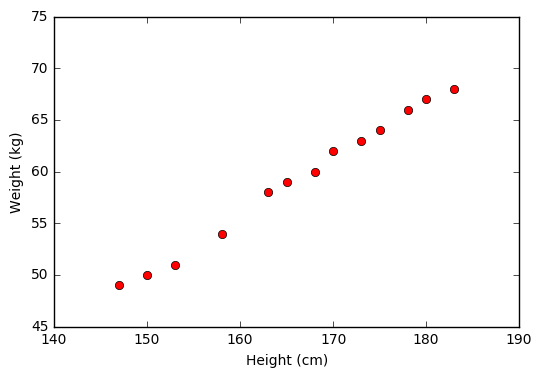
\includegraphics[width = \textwidth]{../LR/output_3_0.png}
 \end{figure}
 
Từ đồ thị này ta thấy rằng dữ liệu được sắp xếp gần như theo 1 đường thẳng, vậy mô hình Linear Regression nhiều khả năng sẽ cho kết quả tốt: 
 
(cân nặng) = \pythoninline{w\_1}*(chiều cao) + \pythoninline{w\_0} 
 
 
\subsection{Nghiệm theo công thức}
 
Tiếp theo, chúng ta sẽ tính toán các hệ số \pythoninline{w_1} và \pythoninline{w_0} dựa vào công thức $(5)$. Chú ý: giả nghịch đảo của một ma trận \pythoninline{A} trong Python sẽ được tính bằng \pythoninline{numpy.linalg.pinv(A)}, \pythoninline{pinv} là từ viết tắt của \textit{pseudo inverse}. 
 
\begin{lstlisting}[language=Python]
# Building Xbar  
one = np.ones((X.shape[0], 1)) 
Xbar = np.concatenate((one, X), axis = 1) 
 
# Calculating weights of the fitting line  
A = np.dot(Xbar.T, Xbar) 
b = np.dot(Xbar.T, y) 
w = np.dot(np.linalg.pinv(A), b) 
print('w = ', w) 
# Preparing the fitting line  
w_0 = w[0][0] 
w_1 = w[1][0] 
x0 = np.linspace(145, 185, 2) 
y0 = w_0 + w_1*x0 
 
# Drawing the fitting line  
plt.plot(X.T, y.T, 'ro')     # data  
plt.plot(x0, y0)               # the fitting line 
plt.axis([140, 190, 45, 75]) 
plt.xlabel('Height (cm)') 
plt.ylabel('Weight (kg)') 
plt.show() 
 
\end{lstlisting}
 
\begin{lstlisting}[language=Python]
w =  [[-33.73541021] 
 [  0.55920496]] 
\end{lstlisting}
 
 


\begin{figure}
	\centering
	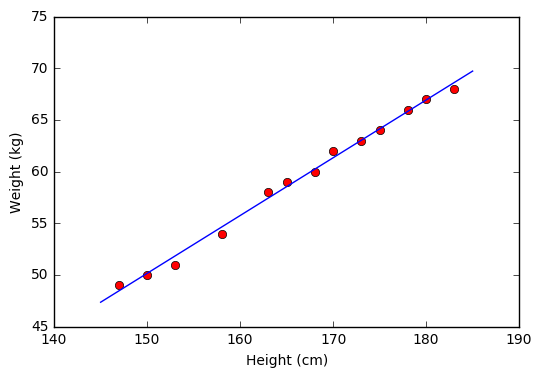
\includegraphics[width = \textwidth]{../LR/output_5_1.png}
\end{figure}
 
Từ đồ thị bên trên ta thấy rằng các điểm dữ liệu màu đỏ nằm khá gần đường thẳng dự đoán màu xanh. Vậy mô hình Linear Regression hoạt động tốt với tập dữ liệu \textit{training}. Bây giờ, chúng ta sử dụng mô hình này để dự đoán cân nặng của hai người có chiều cao 155 và 160 cm mà chúng ta đã không dùng khi tính toán nghiệm. 
 
 
\begin{lstlisting}[language=Python]
y1 = w_1*155 + w_0 
y2 = w_1*160 + w_0 
 
print( 'Predict weight of person with height 155 cm: %.2f (kg), real number: 52 (kg)'  %(y1) ) 
print( 'Predict weight of person with height 160 cm: %.2f (kg), real number: 56 (kg)'  %(y2) ) 
\end{lstlisting}
 
    Predict weight of person with height 155 cm: 52.94 (kg), real number: 52 (kg) 
    Predict weight of person with height 160 cm: 55.74 (kg), real number: 56 (kg) 
 
 
 
Chúng ta thấy rằng kết quả dự đoán khá gần với số liệu thực tế. 
 
 
\subsection{Nghiệm theo thư viện scikit-learn}
 
Tiếp theo, chúng ta sẽ sử dụng thư viện scikit-learn của Python để tìm nghiệm.  
 
 
\begin{lstlisting}[language=Python]
from sklearn import datasets, linear_model 
 
# fit the model by Linear Regression 
regr = linear_model.LinearRegression(fit_intercept=False) # fit_intercept = False for calculating the bias 
regr.fit(Xbar, y) 
 
# Compare two results 
print( 'Solution found by scikit-learn  : ', regr.coef_ ) 
print( 'Solution found by (5): ', w.T) 
\end{lstlisting}
 
\begin{lstlisting}[language=Python]
    Solution found by scikit-learn  :  [[  -33.73541021 0.55920496]] 
    Solution found by (5):  [[  -33.73541021 0.55920496 ]] 
\end{lstlisting}
 
Chúng ta thấy rằng hai kết quả thu được như nhau! (\textit{Nghĩa là tôi đã không mắc lỗi nào trong cách tìm nghiệm ở phần trên}) 
 
\href{https://github.com/tiepvupsu/tiepvupsu.github.io/blob/master/assets/LR/LR.ipynb}{Source code Jupyter Notebook cho bài này.} 
 
 
 
\section{Thảo luận}
 
 
\subsection{Các bài toán có thể giải bằng Linear Regression}
Hàm số $y \approx f(\mathbf{x})= \mathbf{w}^T\mathbf{x}$ là một hàm tuyến tính theo cả $ \mathbf{w}$ và $\mathbf{x}$. Trên thực tế, Linear Regression có thể áp dụng cho các mô hình chỉ cần tuyến tính theo $\mathbf{w}$. Ví dụ: 
$$ 
y \approx w_1 x_1 + w_2 x_2 + w_3 x_1^2 +  w_4 \sin(x_2) + w_5 x_1x_2 + w_0 
$$ 
là một hàm tuyến tính theo $\mathbf{w}$ và vì vậy cũng có thể được giải bằng Linear Regression. Với mỗi dữ liệu đầu vào $\mathbf{x}=[x_1; x_2] $, chúng ta tính toán dữ liệu mới $\tilde{\mathbf{x}} = [x_1, x_2, x_1^2, \sin(x_2), x_1x_2]$ (đọc là \textit{x tilde} trong tiếng Anh) rồi áp dụng Linear Regression với dữ liệu mới này.  
 
Xem thêm ví dụ về \href{http://www.varsitytutors.com/hotmath/hotmath_help/topics/quadratic-regression}{Quadratic Regression} (Hồi Quy Bậc Hai). 
% <div class="imgcap"> 
% <div > 
%     <img src ="http://www.varsitytutors.com/assets/vt-hotmath-legacy/hotmath_help/topics/quadratic-regression/f-qr-1-1.gif"  width = "300"></a> 
% </div> 
% <div class="thecap"> Quadratic Regression (Nguồn: <a href = "http://www.varsitytutors.com/hotmath/hotmath_help/topics/quadratic-regression"> Quadratic Regression</a>) <br></div> 
% </div> 
 
 a figre should be here 
 
\subsection{Hạn chế của Linear Regression}
 
Hạn chế đầu tiên của Linear Regression là nó rất \textbf{nhạy cảm với nhiễu} (sensitive to noise). Trong ví dụ về mối quan hệ giữa chiều cao và cân nặng bên trên, nếu có chỉ 
một cặp dữ liệu \textit{nhiễu} (150 cm, 90kg) thì kết quả sẽ sai khác đi rất nhiều. Xem hình dưới đây: 
% <div class="imgcap"> 
% <img src ="/assets/LR/output_13_1.png" align = "center"> 
% </div> 
 
 \begin{figure}
 	\centering
 	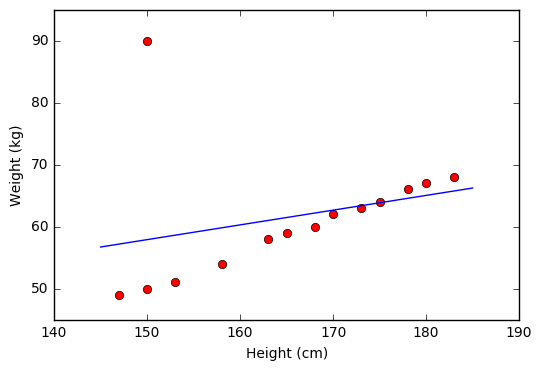
\includegraphics[width = .6\textwidth]{../LR/output_13_1.png}
 \end{figure}
Vì vậy, trước khi thực hiện Linear Regression, các nhiễu (\textit{outlier}) cần 
 phải được loại bỏ. Bước này được gọi là tiền xử lý (pre-processing). 
 
Hạn chế thứ hai của Linear Regression là nó \textbf{không biễu diễn được các mô hình phức tạp}. Mặc dù trong phần trên, chúng ta thấy rằng phương pháp này có thể được áp dụng nếu quan hệ giữa \textit{outcome} và \textit{input} không nhất thiết phải là tuyến tính, nhưng mối quan hệ này vẫn đơn giản nhiều so với các mô hình thực tế. Hơn nữa, chúng ta sẽ tự hỏi: làm thế nào để xác định được các hàm $x_1^2, \sin(x_2), x_1x_2$ như ở trên?! 
 
 
\subsection{Các phương pháp tối ưu}
Linear Regression là một mô hình đơn giản, lời giải cho phương trình đạo hàm bằng 0 cũng khá đơn giản. \textit{Trong hầu hết các trường hợp, chúng ta không thể giải được phương trình đạo hàm bằng 0.} 
 
Nhưng có một điều chúng ta nên nhớ, \textbf{còn tính được đạo hàm là còn có cơ hội}. 
 
 
 
 
\section{Tài liệu tham khảo}
 
1. \href{https://en.wikipedia.org/wiki/Linear_regression}{Linear Regression - Wikipedia} 
2. \href{http://machinelearningmastery.com/simple-linear-regression-tutorial-for-machine-learning/}{Simple Linear Regression Tutorial for Machine Learning} 
3. \href{http://www.sci.utah.edu/~gerig/CS6640-F2012/Materials/pseudoinverse-cis61009sl10.pdf}{Least Squares, Pseudo-Inverses, PCA \& SVD} 


sdfadsf 

% \section{Giới thiệu}
% \label{sec:linearregression_-gioi-thieu}
% % <a name="-gioi-thieu"></a>

% Quay lại [ví dụ đơn giản được nêu trong bài trước]%(/2016/12/27/categories/#regression): một căn nhà rộng $x_1 ~ \text{m}^2$, có $x_2$ phòng ngủ và cách trung tâm thành phố $x_3~ \text{km}$ có giá là bao nhiêu. Giả sử chúng ta đã có số liệu thống kê từ 1000 căn nhà trong thành phố đó, liệu rằng khi có một căn nhà mới với các thông số về diện tích, số phòng ngủ và khoảng cách tới trung tâm, chúng ta có thể dự đoán được giá của căn nhà đó không? Nếu có thì hàm dự đoán $y = f(\mathbf{x}) $ sẽ có dạng như thế nào. Ở đây $\mathbf{x} = [x_1, x_2, x_3] $ là một vector hàng chứa thông tin _input_, $y$ là một số vô hướng (scalar) biểu diễn _output_ (tức giá của căn nhà trong ví dụ này).

% \textbf{Lưu ý về ký hiệu toán học:} \textit{trong các bài viết của tôi, các số vô hướng được biểu diễn bởi các chữ cái viết ở dạng không in đậm, có thể viết hoa, ví dụ $x_1, N, y, k$. Các vector được biểu diễn bằng các chữ cái thường in đậm, ví dụ $\mathbf{y}, \mathbf{x}_1 $. Các ma trận được biểu diễn bởi các chữ viết hoa in đậm, ví dụ $\mathbf{X, Y, W} $.}

% Một cách đơn giản nhất, chúng ta có thể thấy rằng: i) diện tích nhà càng lớn thì giá nhà càng cao; ii) số lượng phòng ngủ càng lớn thì giá nhà càng cao; iii) càng xa trung tâm thì giá nhà càng giảm. Một hàm số đơn giản nhất có thể mô tả mối quan hệ giữa giá nhà và 3 đại lượng đầu vào là: 

% Vũ hữu tiệp 

%%%%%%%%%%%%%%%%%%%%%%%%%%%%%%%%%%%%%%%%%%%
} % End of the \allowdisplaybreak command %
%%%%%%%%%%%%%%%%%%%%%%%%%%%%%%%%%%%%%%%%%%%

\end{document}

